
%% bare_conf.tex
%% V1.4b
%% 2015/08/26
%% by Michael Shell
%% See:
%% http://www.michaelshell.org/
%% for current contact information.
%%
%% This is a skeleton file demonstrating the use of IEEEtran.cls
%% (requires IEEEtran.cls version 1.8b or later) with an IEEE
%% conference paper.
%%
%% Support sites:
%% http://www.michaelshell.org/tex/ieeetran/
%% http://www.ctan.org/pkg/ieeetran
%% and
%% http://www.ieee.org/

%%*************************************************************************
%% Legal Notice:
%% This code is offered as-is without any warranty either expressed or
%% implied; without even the implied warranty of MERCHANTABILITY or
%% FITNESS FOR A PARTICULAR PURPOSE! 
%% User assumes all risk.
%% In no event shall the IEEE or any contributor to this code be liable for
%% any damages or losses, including, but not limited to, incidental,
%% consequential, or any other damages, resulting from the use or misuse
%% of any information contained here.
%%
%% All comments are the opinions of their respective authors and are not
%% necessarily endorsed by the IEEE.
%%
%% This work is distributed under the LaTeX Project Public License (LPPL)
%% ( http://www.latex-project.org/ ) version 1.3, and may be freely used,
%% distributed and modified. A copy of the LPPL, version 1.3, is included
%% in the base LaTeX documentation of all distributions of LaTeX released
%% 2003/12/01 or later.
%% Retain all contribution notices and credits.
%% ** Modified files should be clearly indicated as such, including  **
%% ** renaming them and changing author support contact information. **
%%*************************************************************************


% *** Authors should verify (and, if needed, correct) their LaTeX system  ***
% *** with the testflow diagnostic prior to trusting their LaTeX platform ***
% *** with production work. The IEEE's font choices and paper sizes can   ***
% *** trigger bugs that do not appear when using other class files.       ***                          ***
% The testflow support page is at:
% http://www.michaelshell.org/tex/testflow/



\documentclass[conference]{IEEEtran}
% Some Computer Society conferences also require the compsoc mode option,
% but others use the standard conference format.
%
% If IEEEtran.cls has not been installed into the LaTeX system files,
% manually specify the path to it like:
% \documentclass[conference]{../sty/IEEEtran}





% Some very useful LaTeX packages include:
% (uncomment the ones you want to load)


% *** MISC UTILITY PACKAGES ***
%
%\usepackage{ifpdf}
% Heiko Oberdiek's ifpdf.sty is very useful if you need conditional
% compilation based on whether the output is pdf or dvi.
% usage:
% \ifpdf
%   % pdf code
% \else
%   % dvi code
% \fi
% The latest version of ifpdf.sty can be obtained from:
% http://www.ctan.org/pkg/ifpdf
% Also, note that IEEEtran.cls V1.7 and later provides a builtin
% \ifCLASSINFOpdf conditional that works the same way.
% When switching from latex to pdflatex and vice-versa, the compiler may
% have to be run twice to clear warning/error messages.






% *** CITATION PACKAGES ***
%
%\usepackage{cite}
% cite.sty was written by Donald Arseneau
% V1.6 and later of IEEEtran pre-defines the format of the cite.sty package
% \cite{} output to follow that of the IEEE. Loading the cite package will
% result in citation numbers being automatically sorted and properly
% "compressed/ranged". e.g., [1], [9], [2], [7], [5], [6] without using
% cite.sty will become [1], [2], [5]--[7], [9] using cite.sty. cite.sty's
% \cite will automatically add leading space, if needed. Use cite.sty's
% noadjust option (cite.sty V3.8 and later) if you want to turn this off
% such as if a citation ever needs to be enclosed in parenthesis.
% cite.sty is already installed on most LaTeX systems. Be sure and use
% version 5.0 (2009-03-20) and later if using hyperref.sty.
% The latest version can be obtained at:
% http://www.ctan.org/pkg/cite
% The documentation is contained in the cite.sty file itself.






% *** GRAPHICS RELATED PACKAGES ***
%
\ifCLASSINFOpdf
  \usepackage[pdftex]{graphicx}
  % declare the path(s) where your graphic files are
  % \graphicspath{{../pdf/}{../jpeg/}}
  % and their extensions so you won't have to specify these with
  % every instance of \includegraphics
  % \DeclareGraphicsExtensions{.pdf,.jpeg,.png}
\else
  % or other class option (dvipsone, dvipdf, if not using dvips). graphicx
  % will default to the driver specified in the system graphics.cfg if no
  % driver is specified.
  % \usepackage[dvips]{graphicx}
  % declare the path(s) where your graphic files are
  % \graphicspath{{../eps/}}
  % and their extensions so you won't have to specify these with
  % every instance of \includegraphics
  % \DeclareGraphicsExtensions{.eps}
\fi
% graphicx was written by David Carlisle and Sebastian Rahtz. It is
% required if you want graphics, photos, etc. graphicx.sty is already
% installed on most LaTeX systems. The latest version and documentation
% can be obtained at: 
% http://www.ctan.org/pkg/graphicx
% Another good source of documentation is "Using Imported Graphics in
% LaTeX2e" by Keith Reckdahl which can be found at:
% http://www.ctan.org/pkg/epslatex
%
% latex, and pdflatex in dvi mode, support graphics in encapsulated
% postscript (.eps) format. pdflatex in pdf mode supports graphics
% in .pdf, .jpeg, .png and .mps (metapost) formats. Users should ensure
% that all non-photo figures use a vector format (.eps, .pdf, .mps) and
% not a bitmapped formats (.jpeg, .png). The IEEE frowns on bitmapped formats
% which can result in "jaggedy"/blurry rendering of lines and letters as
% well as large increases in file sizes.
%
% You can find documentation about the pdfTeX application at:
% http://www.tug.org/applications/pdftex





% *** MATH PACKAGES ***
%
\usepackage{amsmath}

%Reference https://www.physicsforums.com/threads/mathbb-stuff-isnt-working.544078/
% A popular package from the American Mathematical Society that provides
% many useful and powerful commands for dealing with mathematics.
%
% Note that the amsmath package sets \interdisplaylinepenalty to 10000
% thus preventing page breaks from occurring within multiline equations. Use:
%\interdisplaylinepenalty=2500
% after loading amsmath to restore such page breaks as IEEEtran.cls normally
% does. amsmath.sty is already installed on most LaTeX systems. The latest
% version and documentation can be obtained at:
% http://www.ctan.org/pkg/amsmath





% *** SPECIALIZED LIST PACKAGES ***
%
%\usepackage{algorithmic}
% algorithmic.sty was written by Peter Williams and Rogerio Brito.
% This package provides an algorithmic environment fo describing algorithms.
% You can use the algorithmic environment in-text or within a figure
% environment to provide for a floating algorithm. Do NOT use the algorithm
% floating environment provided by algorithm.sty (by the same authors) or
% algorithm2e.sty (by Christophe Fiorio) as the IEEE does not use dedicated
% algorithm float types and packages that provide these will not provide
% correct IEEE style captions. The latest version and documentation of
% algorithmic.sty can be obtained at:
% http://www.ctan.org/pkg/algorithms
% Also of interest may be the (relatively newer and more customizable)
% algorithmicx.sty package by Szasz Janos:
% http://www.ctan.org/pkg/algorithmicx




% *** ALIGNMENT PACKAGES ***
%
%\usepackage{array}
% Frank Mittelbach's and David Carlisle's array.sty patches and improves
% the standard LaTeX2e array and tabular environments to provide better
% appearance and additional user controls. As the default LaTeX2e table
% generation code is lacking to the point of almost being broken with
% respect to the quality of the end results, all users are strongly
% advised to use an enhanced (at the very least that provided by array.sty)
% set of table tools. array.sty is already installed on most systems. The
% latest version and documentation can be obtained at:
% http://www.ctan.org/pkg/array


% IEEEtran contains the IEEEeqnarray family of commands that can be used to
% generate multiline equations as well as matrices, tables, etc., of high
% quality.




% *** SUBFIGURE PACKAGES ***
%\ifCLASSOPTIONcompsoc
%  \usepackage[caption=false,font=normalsize,labelfont=sf,textfont=sf]{subfig}
%\else
%  \usepackage[caption=false,font=footnotesize]{subfig}
%\fi
% subfig.sty, written by Steven Douglas Cochran, is the modern replacement
% for subfigure.sty, the latter of which is no longer maintained and is
% incompatible with some LaTeX packages including fixltx2e. However,
% subfig.sty requires and automatically loads Axel Sommerfeldt's caption.sty
% which will override IEEEtran.cls' handling of captions and this will result
% in non-IEEE style figure/table captions. To prevent this problem, be sure
% and invoke subfig.sty's "caption=false" package option (available since
% subfig.sty version 1.3, 2005/06/28) as this is will preserve IEEEtran.cls
% handling of captions.
% Note that the Computer Society format requires a larger sans serif font
% than the serif footnote size font used in traditional IEEE formatting
% and thus the need to invoke different subfig.sty package options depending
% on whether compsoc mode has been enabled.
%
% The latest version and documentation of subfig.sty can be obtained at:
% http://www.ctan.org/pkg/subfig




% *** FLOAT PACKAGES ***
%
%\usepackage{fixltx2e}
% fixltx2e, the successor to the earlier fix2col.sty, was written by
% Frank Mittelbach and David Carlisle. This package corrects a few problems
% in the LaTeX2e kernel, the most notable of which is that in current
% LaTeX2e releases, the ordering of single and double column floats is not
% guaranteed to be preserved. Thus, an unpatched LaTeX2e can allow a
% single column figure to be placed prior to an earlier double column
% figure.
% Be aware that LaTeX2e kernels dated 2015 and later have fixltx2e.sty's
% corrections already built into the system in which case a warning will
% be issued if an attempt is made to load fixltx2e.sty as it is no longer
% needed.
% The latest version and documentation can be found at:
% http://www.ctan.org/pkg/fixltx2e


%\usepackage{stfloats}
% stfloats.sty was written by Sigitas Tolusis. This package gives LaTeX2e
% the ability to do double column floats at the bottom of the page as well
% as the top. (e.g., "\begin{figure*}[!b]" is not normally possible in
% LaTeX2e). It also provides a command:
%\fnbelowfloat
% to enable the placement of footnotes below bottom floats (the standard
% LaTeX2e kernel puts them above bottom floats). This is an invasive package
% which rewrites many portions of the LaTeX2e float routines. It may not work
% with other packages that modify the LaTeX2e float routines. The latest
% version and documentation can be obtained at:
% http://www.ctan.org/pkg/stfloats
% Do not use the stfloats baselinefloat ability as the IEEE does not allow
% \baselineskip to stretch. Authors submitting work to the IEEE should note
% that the IEEE rarely uses double column equations and that authors should try
% to avoid such use. Do not be tempted to use the cuted.sty or midfloat.sty
% packages (also by Sigitas Tolusis) as the IEEE does not format its papers in
% such ways.
% Do not attempt to use stfloats with fixltx2e as they are incompatible.
% Instead, use Morten Hogholm'a dblfloatfix which combines the features
% of both fixltx2e and stfloats:
%
% \usepackage{dblfloatfix}
% The latest version can be found at:
% http://www.ctan.org/pkg/dblfloatfix




% *** PDF, URL AND HYPERLINK PACKAGES ***
%
%\usepackage{url}
% url.sty was written by Donald Arseneau. It provides better support for
% handling and breaking URLs. url.sty is already installed on most LaTeX
% systems. The latest version and documentation can be obtained at:
% http://www.ctan.org/pkg/url
% Basically, \url{my_url_here}.




% *** Do not adjust lengths that control margins, column widths, etc. ***
% *** Do not use packages that alter fonts (such as pslatex).         ***
% There should be no need to do such things with IEEEtran.cls V1.6 and later.
% (Unless specifically asked to do so by the journal or conference you plan
% to submit to, of course. )


% correct bad hyphenation here
\hyphenation{op-tical net-works semi-conduc-tor}


\begin{document}
%
% paper title
% Titles are generally capitalized except for words such as a, an, and, as,
% at, but, by, for, in, nor, of, on, or, the, to and up, which are usually
% not capitalized unless they are the first or last word of the title.
% Linebreaks \\ can be used within to get better formatting as desired.
% Do not put math or special symbols in the title.
\title{Accelerate Evaluation for Lane Change Scenario using Gaussian Mixture Model and Monotonic Rare-event Set Learning}


% author names and affiliations
% use a multiple column layout for up to three different
% affiliations
\author{\IEEEauthorblockN{Zhiyuan Huang}
\IEEEauthorblockA{Department of Industrial and\\Operations Engineering\\
University of Michigan\\}
\and
\IEEEauthorblockN{Ding Zhao}
\IEEEauthorblockA{University of Michigan\\
Transportation Research Institude}
\and
\IEEEauthorblockN{James Kirk\\ and Montgomery Scott}
\IEEEauthorblockA{Starfleet Academy\\
San Francisco, California 96678--2391\\
Telephone: (800) 555--1212\\
Fax: (888) 555--1212}}

% conference papers do not typically use \thanks and this command
% is locked out in conference mode. If really needed, such as for
% the acknowledgment of grants, issue a \IEEEoverridecommandlockouts
% after \documentclass

% for over three affiliations, or if they all won't fit within the width
% of the page, use this alternative format:
% 
%\author{\IEEEauthorblockN{Michael Shell\IEEEauthorrefmark{1},
%Homer Simpson\IEEEauthorrefmark{2},
%James Kirk\IEEEauthorrefmark{3}, 
%Montgomery Scott\IEEEauthorrefmark{3} and
%Eldon Tyrell\IEEEauthorrefmark{4}}
%\IEEEauthorblockA{\IEEEauthorrefmark{1}School of Electrical and Computer Engineering\\
%Georgia Institute of Technology,
%Atlanta, Georgia 30332--0250\\ Email: see http://www.michaelshell.org/contact.html}
%\IEEEauthorblockA{\IEEEauthorrefmark{2}Twentieth Century Fox, Springfield, USA\\
%Email: homer@thesimpsons.com}
%\IEEEauthorblockA{\IEEEauthorrefmark{3}Starfleet Academy, San Francisco, California 96678-2391\\
%Telephone: (800) 555--1212, Fax: (888) 555--1212}
%\IEEEauthorblockA{\IEEEauthorrefmark{4}Tyrell Inc., 123 Replicant Street, Los Angeles, California 90210--4321}}




% use for special paper notices
%\IEEEspecialpapernotice{(Invited Paper)}




% make the title area
\maketitle

% As a general rule, do not put math, special symbols or citations
% in the abstract
\begin{abstract}
The abstract goes here.
\end{abstract}

% no keywords




% For peer review papers, you can put extra information on the cover
% page as needed:
% \ifCLASSOPTIONpeerreview
% \begin{center} \bfseries EDICS Category: 3-BBND \end{center}
% \fi
%
% For peerreview papers, this IEEEtran command inserts a page break and
% creates the second title. It will be ignored for other modes.
\IEEEpeerreviewmaketitle



\section{Introduction}
% no \IEEEPARstart

AV has been popular, evaluation important. Lane change scenario is interested to us, because (lane change crash data, times, percentage).

Other approaches.

In (REF), we proposed the Accelerated Evaluation concept and used the procedure to evaluate Automated Vehicles crash risks in natural driving environment. We mainly explored the application on models of interaction between AVs and human-controlled vehicles. In (REF), we modeled the frontal crash with a lead vehicle(HV or AV) using single variable Gaussian process. We also explored different approaches to tackle the evaluation of lane change scenario(REF). 

In previous work, the results are based on the independence of variables(name?). We managed to decompose the density distribution and model the randomness using single variate distributions.  In (REF), we used single parametric distribution to model the variables and we proposed the piecewise mixture distribution (REF) to increase the accuracy of model fitting. Cross entropy method was used to construct the importance sampling distribution. Since the independence of variables is concluded from data observation, it is not strictly proved. Ignoring the dependence between variables might lead to some estimation error. Moreover, the independence of variables is not a general condition. The requirement of independence limits the application popularity(better word needed) of the Accelerated Evaluation.

In this paper, we proposed an Accelerated Evaluation procedure using Gaussian Mixture Model for lane change scenario. (dependency) The GMM can model the dependency between variables. (accuracy) By increasing the number of components in GMM, the fitting...

Due to numbers of parameter, using cross entropy to construct IS distribution can be inefficient. (explain) We develop a new procedure based on the monotonicity property of the lane change problem. We derive a rare-event set learning procedure to construct IS distribution using both monotonicity property of rare-event sets and efficiency of change of measure for Gaussian distributions.

provide an upper and lower bound for the estimation.

Section \ref{sec:lane} reviews the setting of the lane change scenario. In Section \ref{sec:gmm}, we review the truncated GMM fitting. The definition of monotonicity rare-event sets and the set learning algorithm are present in Section \ref{sec:monotone}. We introduce how to constructing an efficient Important Sampling distribution for GMM in Section \ref{sec:is} and show the specific approach for monotonicity rare-events(monotone?). We present the simulation results for the lane change scenario in Section \ref{sec:result}. Section \ref{sec:conclusion} concludes the paper.

\section{The Lane Change Scenario}\label{sec:lane}

The lane change scenario studied in this paper is the defined as the following: a human-controlled vehicle driving in front of an automated vehicle start to cut in the lane where the automated vehicle is running. We want to evaluate the risk of crash in this scenario. Since the initial condition for the scenario is controlled by the AV, we can take it as a random environment. Then we can use the Automated Vehicle model to simulate the output (crash or not) for a given initial condition.

To model the initial condition of lane changes, we extracted data from the Safety Pilot Model Deployment (SPMD) database (Bezzina2014). The database includes over 2 million miles of vehicle driving data collected from 98 cars over 3 years. we identify 403,581 lane change events and use 173,692 events with a negative range rate to build statistical models. Three key variables can capture the effects of gap acceptance of the lane changing vehicle: velocity of the lead vehicle ($v_L$), range to the lead vehicle ($R_L$) and time to collision ($TTC_L$). $TTC_L$ was defined as:
\begin{equation}
	TTC_L=- \frac{R_L}{\dot{R_L}},
\end{equation}
where $\dot{R_L}$ is the relative speed.  

The simulation of Automated Vehicle model is based on Adaptive Cruise Control (ACC) and Autonomous Emergency Braking (AEB) (Ulsoy2012a) regarding the surrounding environment. With an initial condition, the simulator returns an output of the scenario. We can considered as an event indicator function $I_\varepsilon(x)$ that returns $1$ (crash) or $0$ (safe) depending on the event of interest.



\section{Gaussian Mixture Model Fitting}\label{sec:gmm}

In this section, we review the truncated GMM fitting studied by Lee and Scott (REF). 

The fitting of Gaussian Mixture Model is well studied and generally used. In the lane change scenario, the data can be considered as truncated. For instance, the range of two cars cannot be negative. For this reason, we use the truncated GMM to model the initial condition. 


For a $d$ dimensional dataset with truncated as a hyper-rectangle with vertices $s$ and $t$, observations $y^n$ satisfies $s\leq y^n \leq t$. Note that we can have $s_i=-\infty$ or $t_i=\infty$, which indicates the $i$th coordinate is not truncated below or above.

For a truncated GMM with $K$ components, we use observation to estimate parameters in \begin{equation}
g(y)=\sum_{k=1}^{K} \eta_k g_k(y),
\end{equation}
where $\eta_k$ is the mixing weights, $g_k$ is truncated Gaussian with support $[s,t]$, mean $\mu_k$ and covariance $\Sigma_k$. Similarly as the vanilla GMM fitting, we use an EM algorithm to estimate the parameters. With a proper initial value for the estimated parameters, we use the following algorithm to iterate for converged estimators.

The E-step is:
\begin{equation}
\langle z_k^n \rangle =\frac{\eta_k g_k(y^n)}{\sum_{l} \eta_l g_l(y^n)},
\end{equation}
where we define $\langle z_k^n \rangle = p[z_k^n=1|y^n]$ to denote the probability that $y^n$ is generated from the $k$th component.

The M-step is also similar to the vanilla GMM fitting except some correction terms:
\begin{equation}
\hat{\eta}_k =\frac{1}{N} \sum_n \langle z_k^n \rangle ,
\end{equation}
\begin{equation}
\hat{\mu}_k =\frac{\sum_n \langle z_k^n \rangle y^n}{\sum_n \langle z_k^n \rangle} - m_k ,
\end{equation}
\begin{equation}
\hat{\Sigma}_k =\frac{\sum_n \langle z_k^n \rangle (y^n-\hat{\mu}_k)(y^n-\hat{\mu}_k)^T}{\sum_n \langle z_k^n \rangle}+ H_k ,
\end{equation}
where\begin{equation}
m_k=\mathcal{M}^1(0,\Sigma_k;[s-\mu_k,t-\mu_k]),
\end{equation}
\begin{equation}
H_k=\Sigma_k-\mathcal{M}^2(0,\Sigma_k;[s-\mu_k,t-\mu_k]).
\end{equation}
$\mathcal{M}^1(\mu,\Sigma;[a,b])$ and $\mathcal{M}^2(\mu,\Sigma;[a,b])$ denote the first and second moment of truncated Gaussian distribution with truncating vertices $a,b$, mean $\mu$ and covariance $\Sigma$.

The choice of number of components $K$ can be determined by some criterion for goodness of fitting, for example, we can use the Bayesian Information Criterion (BIC).

\section{Importance Sampling Distribution for Gaussian Mixture Models}\label{sec:is}
In this section, we first review the concept of Importance Sampling and some known Importance Sampling schemes for rare events with Gaussian distribution. We derive the scheme for GMM based on these background knowledge.
\subsection{Importance Sampling for Gaussian Distribution}
Importance Sampling is a technique to reduce the variance in simulation. 

Consider a random vector $x$ with distribution $F$ and a rare event set $\varepsilon \subset \Omega$ on sample space $\Omega$. Our goal is to estimate the probability of the rare event \begin{equation}
{P}(X \in \varepsilon)=E[I_\varepsilon(X)]=\int I_\varepsilon(x) dF,
\end{equation} where the event indicator function is defined as\begin{equation}
	I_\varepsilon(x)=\begin{cases} 1 & x \in \varepsilon.\\
0 & otherwise.\end{cases}
\end{equation}

The crude Monte Carlo using the sample mean of $I_\varepsilon(x)$ \begin{equation}
	\hat{P}(X \in \varepsilon) = \frac{1}{N} \sum_{n=1}^N I_\varepsilon(X_n),
\end{equation}
where $X_i$'s are drawn from distribution $F$.

The Importance Sampling \cite{Bucklew2004a} technique is derived from\begin{equation}
	E[I_\varepsilon(X)]=\int I_\varepsilon(x) dF = \int I_\varepsilon(x) \frac{dF}{dF^*} dF^* ,
\end{equation}
which gives the estimator using the sample mean of the above expectation (use ref) \begin{equation}
	\hat{P}(X \in \varepsilon) = \frac{1}{N} \sum_{n=1}^N I_\varepsilon(X_n) \frac{dF}{dF^*},
\end{equation}
where $X_i$'s are generated from $F^*$, which has the same support with $F$. We note that this is an unbiased estimation of ${P}(X \in \varepsilon) $. By appropriately selecting $F^*$, the evaluation procedure obtains an estimation with smaller variance. $F^*$ is called the IS distribution. For simplicity, we define the likelihood function \begin{equation}
L(x)=\frac{dF(x)}{dF^*(x)}.
\end{equation}

The analysis of asymptotic efficiency (REF) is a benchmark to determine whether an IS distribution is proper. Let $Z=L(x) I_\varepsilon(x)$ be an IS estimator, it is weakly efficient if \begin{equation}
\lim_{\varepsilon \rightarrow \infty} \frac{\log \left( E_{F^*} [Z^2] \right)}{\log \left( E_{F^*}[Z] \right)} = 2,
\end{equation}
where $\varepsilon \rightarrow \infty$ denotes that the rare event set $\varepsilon$ diverges to $\infty$ in a suitable sense (e.g., $\inf_{x\in \varepsilon}  \| x\|_2 \rightarrow \infty $).

When $x$ follows Gaussian distribution with mean $\mu$ and covariance matrix $\Sigma$ and the rare event set $\varepsilon$ satisfies certain assumptions, there is a simple scheme that obtains an weakly efficient IS distribution. Here, we introduce the scheme with assumptions satisfied in the lane change scenario.

For a convex set rare event set $\varepsilon$, we define \begin{equation}
	a^*=\arg \max_{a\in \varepsilon} \phi(a;\mu,\Sigma)
\end{equation}
to be the dominating point of $\varepsilon$ on $\phi(\cdot;\mu,\Sigma)$, where $\phi(\cdot;\mu,\Sigma)$ is the density function for Gaussian distribution with mean $\mu$ and covariance matrix $\Sigma$. The dominating point contributes the highest density among all points in $\varepsilon$. By shifting the mean $\mu$ of the Gaussian distribution to $a^*$, we can obtain an IS distribution that provides a weakly effecient estimator for $P(x \in \varepsilon)$ (REF).

\subsection{IS Scheme for Gaussian Mixture Model and Union of Convex Rare Event Sets}
Based on the IS scheme for Guassian distribution on convex rare event set, we propose an IS scheme for Gaussian Mixture Model on the union of convex rare event sets. 
  
Assume $x$ follows a Gaussian Mixture Model with $k$ components, the density of $x$ is \begin{equation}
	f(x)=\sum_{i=1}^{k}p_i \phi(x;\mu_i,\Sigma_i).
	\label{eq:gmm_density}
\end{equation}
The rare event set $\varepsilon$ is consisted with $l$ convex sets, we denote as $\varepsilon = \cup_{j=1}^{l} \varepsilon_j$.

For each convex set $\varepsilon_j$, we find the dominating point of $\varepsilon_j$ on the Gaussian component $\phi(x;\mu_i,\Sigma_i)$ by \begin{equation}
	a_{ij}^*=\arg \max_{a\in \varepsilon_j} \phi(a;\mu_i,\Sigma_i).
\end{equation}
We propose to use the IS distribution as following:\begin{equation}
	f^*(x)=\sum_{i=1}^{k} \sum_{j=1}^{l} p_i q_j \phi(x;a_{ij},\Sigma_i),
\end{equation}
where the $q_j$ can be arbitrary positive number that satisfies $\sum_{j=1}^{l} q_j=1$. We can use $q_j={1}/{l}$.


\section{Monotonic Rare Event Sets Learning}\label{sec:monotone}
In this section, we first define the monotonicity for rare event sets. Then we propose a learning algorithm to obtain an outer approximation set and an inner approximation set of a rare event set based on the monotonic property.

the result set is a strict inner/outer set, can provide bound for the estimation.
\subsection{Definition of Monotonic Rare Event Sets}
For a rare event set $\varepsilon$ on $d$ dimensional space, if $x_1 \in \varepsilon$ and $x_1 \leq x_2$ (or $x_1 \geq x_2$) implies that $x_2 \in \varepsilon$, we call the set $\varepsilon$ non-decreasing (or non-increasing).

For example, in the lane change scenario, if a crash occurs for initial condition $(v_L, TTC_L, R_L)$, then if any of these variable is smaller, we can determine that a crash will happen. The set for crash is non-increasing. This can be explained intuitively, because a smaller $v_L$, $TTC_L$ and $R_L$ means that there is less room for the following Automated Vehicle to make adjustment.

\begin{figure}[t]
	\centering
	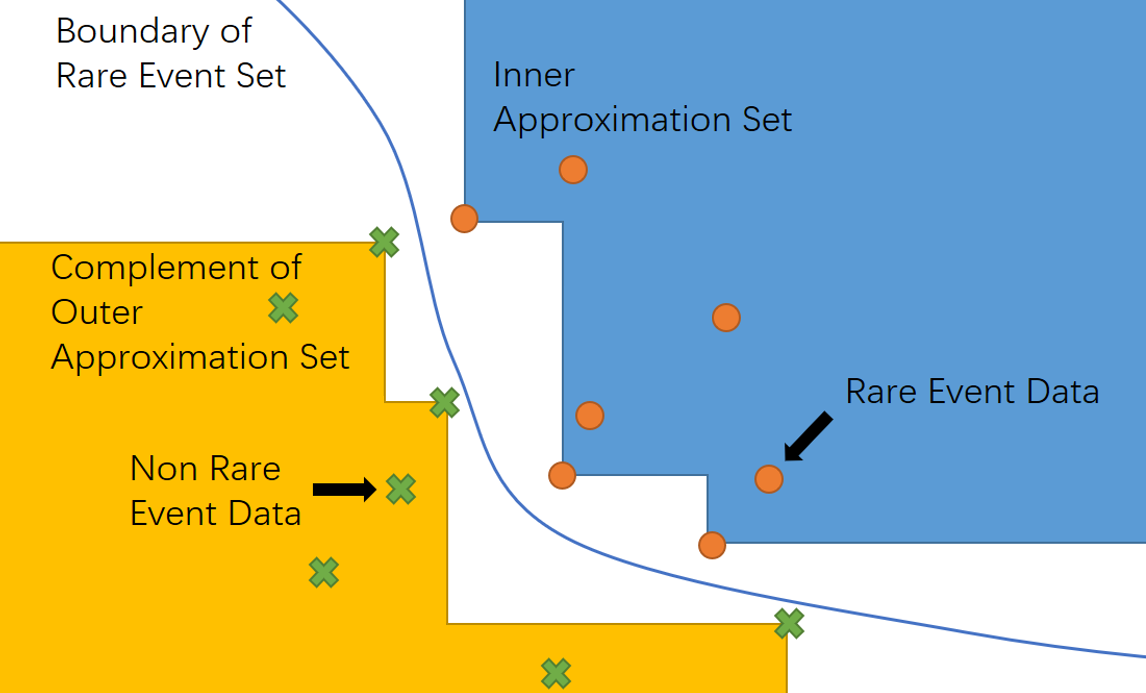
\includegraphics[width=0.8\linewidth]{monotonic_figure.png}
	\caption{An illustration of monotonic set learning.}
	\label{fig:mono}
\end{figure}


\subsection{Learning Algorithm}

Since our goal for learning the approximation set of rare event is to construct an IS distribution, we want the approximated set to satisfy the assumption in the scheme we proposed in Section \ref{sec:is}. Therefore, we want the approximation set to be an union of convex sets.

Let us consider a non-decreasing rare event set $\varepsilon $ on a $d$ dimensional space. We denote $\mathcal{S}_1=\{a^1,...,a^{n_1}\}$ as the observed data in the rare event set and $\mathcal{S}_0=\{b^1,...,b^{n_0}\}$ as the observed data not contained by the rare event set. We use $\mathcal{S}_1$ to construct an inner approximation set $\underline{\varepsilon}$ and use $\mathcal{S}_0$ to construct an outer approximation set $\bar{\varepsilon}$. 

For each data point $a_i$ in $\mathcal{S}_1$, we construct a set $\mathcal{I}_i=\{x:x \geq a_i\}$. By the definition of non-decreasing set, we have $\mathcal{I}_i \subset \epsilon$. Therefore, we have $\underline{\varepsilon}= \cup_{i=1}^{n_1} \mathcal{I}_i \subset \epsilon$ as the inner approximation set of $\varepsilon $.


 For each data point $b_j$ in $\mathcal{S}_0$, we construct sets $\mathcal{O}_{jk}=\{x:x^k \geq b^k_j\} $ for $k=1,...,d$, where $x^k$ denotes the $k$th element in $x$ and $b^k_j$ denotes the $k$th element in $b_j$. We have $\epsilon \subset \cup_{k=1}^{d} \mathcal{O}_{jk}$, which indicates that $\epsilon \subset \cup_{j=1}^{n_0} \cup_{k=1}^{d} \mathcal{O}_{jk}$. We define $\bar{\varepsilon} = \cup_{j=1}^{n_0} \cup_{k=1}^{d} \mathcal{O}_{jk}$ as the outer approximation set of $\varepsilon $.

We note that $\mathcal{I}_i$'s and $\mathcal{O}_{jk}$'s are convex, the approximation sets are unions of convex sets. We also note that using the minimums of $\mathcal{S}_1$ or maximums of $\mathcal{S}_0$ (also known as Pareto fronts) of the dataset provides the same inner or outer approximation set (minimum and maximum in a multi objective optimization sense.)

Additionally, to use the result for non-decreasing sets, we can simply flip all coordinates of data (take negative value) when we have a non-increasing set. For sets that is non-decreasing on some of the coordinates and non-increasing on the rest coordinates, we can flip the value of data those non-increasing coordinates. The approximation sets obtained will still be union of convex sets after flipping any coordinate.

\section{Scheme for Constructing IS Distribution for A Gaussian Mixture Model with A Monotonic Rare Event Set}

Combining the discussion in Sections \ref{sec:is} and \ref{sec:monotone}, we propose an iterated procedure that provides IS distributions for a Gaussian Mixture Model with a monotonic rare event set.

Here, we consider a non-decreasing rare event set $\varepsilon$ on $d$ dimensional space and the variable vector $x$ is generated from a $k$ components GMM with density (\ref{eq:gmm_density}). To clarify the notations, for each Gaussian component $i$, we construct a set of dominating points $\mathcal{A}_I^i$ using the inner approximation set $\underline{\varepsilon}$ and $\mathcal{A}_O^i$ using the inner approximation set $\bar{\varepsilon}$ for $i=1,...,k$ . $|\mathcal{A}|$ denotes the number of elements in the set $\mathcal{A}$. $\underline{\varepsilon}$ and $\bar{\varepsilon}$ are constructed based on $\mathcal{S}_1$, which contains the minimums of observed data in $\varepsilon$, and $\mathcal{S}_0$, which contains the maximums of observed data that not in $\varepsilon$. The procedure iterates to update these sets, which will provide two IS distributions $f^*_I$ and $f^*_O$ based on the inner approximation and the outer approximation of $\varepsilon$ respectively.

The procedure is present as the following:
\begin{enumerate}
\item Initialize $A^i_I=A^i_O=\{\mu_i\}$ and $\mathcal{S}_1=\mathcal{S}_0=\emptyset$.
\item Construct the sampling distribution\begin{equation}
f^*_I(x)=\sum_{i=1}^{k} \sum_{a \in \mathcal{A}^i_I} p_i \frac{1}{|\mathcal{A}^i_I|} \phi(x;a,\Sigma_i)
\end{equation} and \begin{equation}
f^*_O(x)=\sum_{i=1}^{k} \sum_{a \in \mathcal{A}^i_O} p_i \frac{1}{|\mathcal{A}^i_O|} \phi(x;a,\Sigma_i)
\end{equation} \label{step:start}

\item Sample $N$ data points $D=\{x_1,...,x_N\}$ from the density \begin{equation}
f(x)=\rho f^*_I(x) +(1-\rho) f^*_O(x),
\end{equation}
where we can pick $\rho$ on $[0,1]$. We can use $\rho= 1/2 \ I_{\{\mathcal{S}_1 \neq \{\mu_i\}\}}.$

\item Input $D$ to the simulator $I_\varepsilon(x)$ and use the outcome to update $S_1$ and $S_0$. We add the new data points to $S_1$ and $S_0$ regarding the outcome of $I_\varepsilon(x)$. Then we discard non-minimum data points in $S_1$ and non-maximum data points in $S_0$.

\item For each Gaussian component $i$, we use each data points $a \in S_1$ to solve \begin{equation}
\max_x \ \phi(x;\mu_i,\Sigma_i)\ \text{subject to } x\geq a. \label{eq:opt_nominate_1}
\end{equation}
We obtain $|S_1|$ solutions and the solution set is our new $\mathcal{A}^i_I$.

\item For each Gaussian component $i$, we use each data points $b \in S_0$ to solve \begin{equation}
\max_x \ \phi(x;\mu_i,\Sigma_i)\ \text{subject to } x_m\geq b_m, \label{eq:opt_nominate_0}
\end{equation}
for $m=1,...,d$. $ x_m\geq b_m$ denotes the $m$th element of $x$ is greater or equals to the $m$th element of $b$.
We obtain $d|S_0|$ solutions and the solution set is our new $\mathcal{A}^i_O$. \label{step:end}

\item Iterate from \ref{step:start}) to \ref{step:end}).

\end{enumerate}







Truncated: no asymptotic on truncated coordinate.

\section{Simulation Analysis on Lane Change Scenario}\label{sec:result}

In this section, we present the result in GMM fitting, IS distribution constructed and show simulation results.

\subsection{Truncated Gaussian Mixture Model Fitting}
Since the truncated Gaussian Mixture Model fitting is a trivial fitting exercise, here we only present the selection of the number of components $K$. Fig. \ref{fig:bic} shows the BIC regards to different $K$. We could observe that we obtain a local minimum at $K=9$, where it means that the model with $K=9$ provides a balance between the number of parameters and the fitting. 

We note that the different scale of the variables might cause some numerical issues in implementing the algorithm presented in Section \ref{sec:gmm}, we can normalize (subtract by marginal mean and then divided by marginal standard deviation) the data before we fit the model.

\begin{figure}[t]
	\centering
	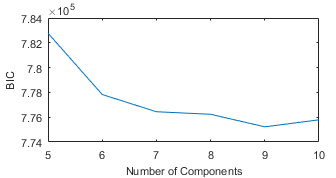
\includegraphics[width=\linewidth]{BIC_plot.png}
	\caption{The BIC regarding to different number of components $K$.}
	\label{fig:bic}
\end{figure}

% conference papers do not normally have an appendix
In the lane change scenario, since the variables are truncated, we need to make some adjustment in the procedure. Note that if we directly use (\ref{eq:opt_nominate_1}) and (\ref{eq:opt_nominate_0}) for truncated variables, we might obtain a solution that out of the range of interest. In that case, the corresponding sampling distribution component 

\section{Conclusion}\label{sec:conclusion}
% use section* for acknowledgment
\section*{Acknowledgment}


The authors would like to thank...





% trigger a \newpage just before the given reference
% number - used to balance the columns on the last page
% adjust value as needed - may need to be readjusted if
% the document is modified later
%\IEEEtriggeratref{8}
% The "triggered" command can be changed if desired:
%\IEEEtriggercmd{\enlargethispage{-5in}}

% references section

% can use a bibliography generated by BibTeX as a .bbl file
% BibTeX documentation can be easily obtained at:
% http://mirror.ctan.org/biblio/bibtex/contrib/doc/
% The IEEEtran BibTeX style support page is at:
% http://www.michaelshell.org/tex/ieeetran/bibtex/
%\bibliographystyle{IEEEtran}
% argument is your BibTeX string definitions and bibliography database(s)
%\bibliography{IEEEabrv,../bib/paper}
%
% <OR> manually copy in the resultant .bbl file
% set second argument of \begin to the number of references
% (used to reserve space for the reference number labels box)
\begin{thebibliography}{1}

\bibitem{IEEEhowto:kopka}
H.~Kopka and P.~W. Daly, \emph{A Guide to \LaTeX}, 3rd~ed.\hskip 1em plus
  0.5em minus 0.4em\relax Harlow, England: Addison-Wesley, 1999.

\end{thebibliography}




% that's all folks
\end{document}


